\section{Modelo de caminos.}



Suponga  la  siguiente  situación,  una  persona se encuentra de paseo en una ciudad y está interesada en ir de la esquina A hasta la esquina B por la ruta más corta posible, tal como lo muestra la siguiente figura:

\begin{center}

    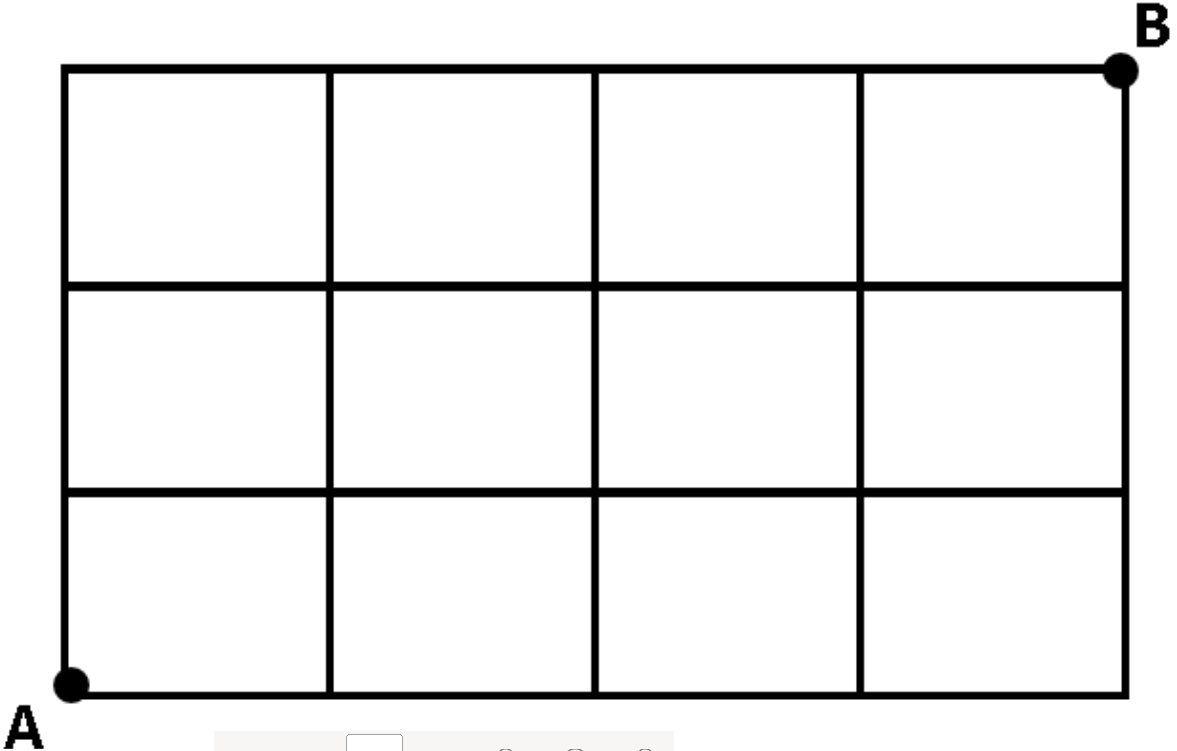
\includegraphics[scale=0.25]{Imagenes/IMG4/caminos_1.png}\\
    Figura 1
\end{center}

¿De cuántas formas podemos realizar dicho recorrido? Hay 35 maneras de hacerlo ¡compruébelo!



En primer lugar,  

En general, consideremos una cuadrícula de dimensión $k \times n$, como la siguiente:

\begin{center}
    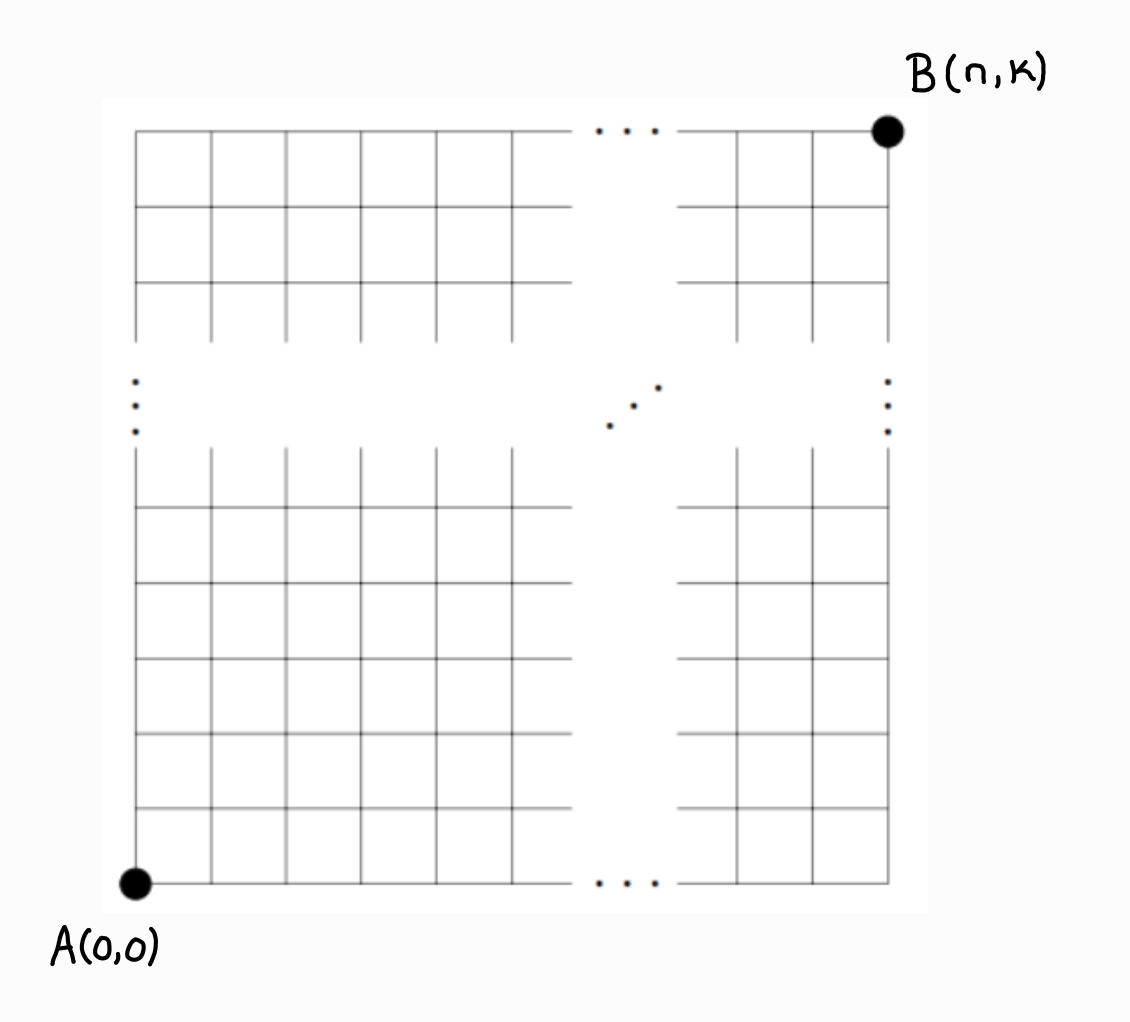
\includegraphics[scale=0.2]{Imagenes/IMG4/caminos_2.jpg}
\end{center}

Queremos saber la cantidad de caminos de longitud mínima que llevan del punto A al punto B notemos que los caminos de longitud mínima deben estar formados por $n$ movimientos a la derecha y $k$ hacia arriba. Así el problema se traduce a un problema de decisiones, en cada punto de la cuadrícula se debe decidir si se hará un movimiento a la derecha $\rightarrow$ o hacia arriba $\uparrow$ y tenemos obligatoriamente que escoger $n$ veces movimientos a la derecha y $k$ veces arriba. Consideremos la función biyectiva $$\delta : \{ \rightarrow, \uparrow\} \longrightarrow \{0,1\}$$ donde $\delta(\rightarrow)=1$ y $\delta(\uparrow)=0$. Un camino en la cuadrícula se puede ver como una lista de la forma $\{ \rightarrow, \rightarrow, \uparrow, \cdots \uparrow\}$ donde $\rightarrow$ aparece $n$ veces y $\uparrow$ $k$ veces. Mediante la función anterior cada camino queda representado como una cadena de ceros y unos de longitud $n+k$ con $n$ unos; por ejemplo para un camino de la cuadrícula de la figura 1 tenemos

$$\{ \rightarrow, \rightarrow, \uparrow, \uparrow, \rightarrow, \uparrow, \rightarrow\}\longrightarrow \{ \delta(\rightarrow), \delta(\rightarrow), \delta(\uparrow), \delta(\uparrow), \delta(\rightarrow), \delta(\uparrow), \delta(\rightarrow)\}=\{1,1,0,0,1,0,1\}.$$

Así por el principio de correspondencia contar el total de caminos de la cuadrícula anterior equivale a contar el total de cadenas de ceros y unos de longitud $n+k$ con $n$ unos lo cual es $$\binom{n+k}{k}$$


Regresando a la figura 1, hay 35 caminos dado que tenemos 4 opciones obligatorias a la derecha y 3 opciones obligatorias hacia arriba, así el total de caminos es $\displaystyle\binom{7}{4}$. 



\section{Problemas.}


\begin{problema}
    Considerar la cuadrícula y que solo se permiten movimientos hacia la derecha o hacia arriba. Responder cuántos caminos de longitud mínima llevan:

    \begin{center}
        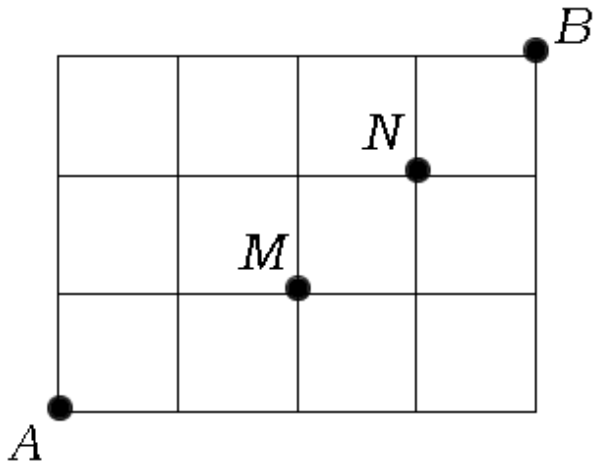
\includegraphics[scale=0.4]{Imagenes/IMG3/Caminos4.png}
    \end{center}

    \renewcommand{\theenumi}{\alph{enumi})}
    \begin{enumerate}      

    
        \item De A a M.
        \item De M a B.
        \item De A a B pasando por M.
        \item De A a B pasando por N.
        \item De A a B pasando por M y N.
        \item De A a B pasando por M o N.
        \item De A a B y no pasan ni por M ni por N.
    \end{enumerate}

\renewcommand{\theenumi}{\arabic{enumi}}

    
\end{problema}


\begin{problema}
    Considerando la siguiente cuadrícula responde a las siguientes preguntas:

    \begin{figure}[H]
        \centering
        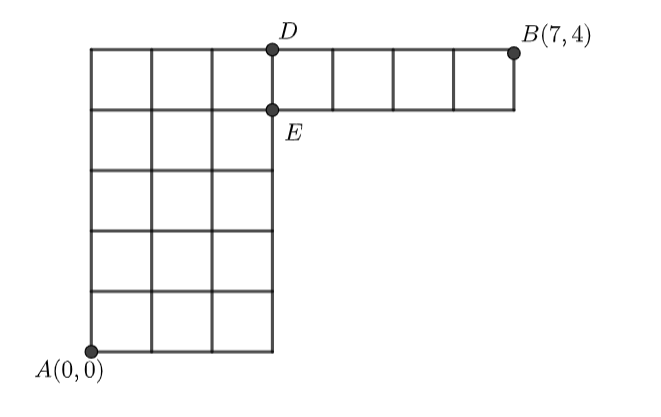
\includegraphics[scale=0.6]{Imagenes/IMG3/Cuadricula_1.png}
    \end{figure}

    \renewcommand{\theenumi}{\alph{enumi})}
    \begin{enumerate}
        \item ¿Cuántos caminos (de longitud mínima) hay de A a B?

        \item Considerando los caminos del literal $a)$ ¿Cuántos pasan por $E$ y $D$?

        \item ¿Cuántos de los caminos del literal $a)$ pasan por $E$ ó por $D$?
    \end{enumerate}
    
\end{problema}
\renewcommand{\theenumi}{\arabic{enumi}}




\begin{problema}
    En cada una de las cuadrículas, expresar usando números combinatorios (no es necesario calcularlos) ¿cuántos caminos de longitud mínima comienzan en el punto A y terminan en el punto B?

    \begin{center}
        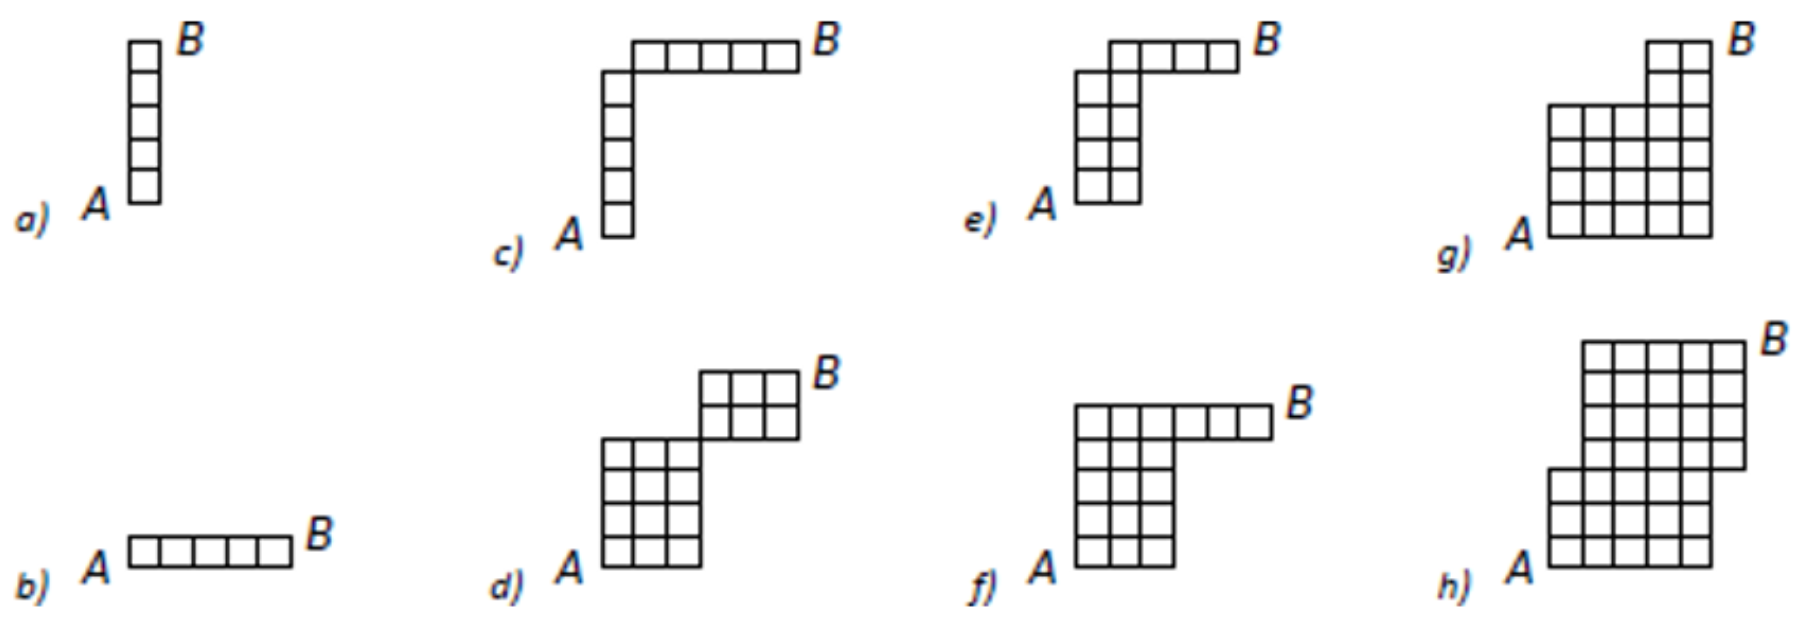
\includegraphics[scale=0.6]{Imagenes/IMG3/Caminos3.png}
    \end{center}
    
\end{problema}

\begin{problema}
    Dibujar una cuadrícula cuya cantidad de caminos sea igual a la especificada en cada caso.

    \renewcommand{\theenumi}{\alph{enumi})}
    \begin{enumerate}

        

        \item $\binom{7}{3}$
        \item $\binom{7}{3}^2$
        \item $\binom{5}{3}\binom{6}{2}$
        \item $\binom{5}{2}\binom{6}{4}$
    \end{enumerate}
    \renewcommand{\theenumi}{\arabic{enumi}}
\end{problema}



\begin{problema}
    Demostrar usando el modelo de caminos que cada una de las siguientes igualdades son identidades. Sugerencia: Construir una cuadrícula adecuada adecuada.


    \renewcommand{\theenumi}{\alph{enumi})}
    \begin{enumerate}

        \item $\binom{6}{3}=\binom{4}{1}\binom{2}{2}+\binom{4}{2}\binom{2}{1}+\binom{4}{3}\binom{2}{0}$  

        
        %\item $C^6_3=C^4_1C_2^2+C_2^4C_1^2+C_3^4C_0^2$


        \item $\binom{6}{3}=\binom{3}{0}\binom{3}{3}+\binom{3}{1}\binom{3}{2}+\binom{3}{3}\binom{3}{0}$

        
        
        %\item $C_3^6=C_0^3C_3^3+C_1^3C_2^3+C_3^3C_0^3$


        \item $\binom{12}{2}=2\binom{6}{2}+6^2$


        
        %\item $C_2^{12} = 2C_2^6+6^2$ (sugerencia: Demostrar que el lado derecho se puede escribir como $C_0^6C_2^6+C_1^6C_1^6+C_2^6C_0^6$)
    \end{enumerate}
\end{problema}

\renewcommand{\theenumi}{\arabic{enumi}}




\begin{problema}
    Para cada una de Determina el númelas siguienero de caminos de A hasta B, con movimientos hacia abajo y a la derecha

    
    \begin{center}
        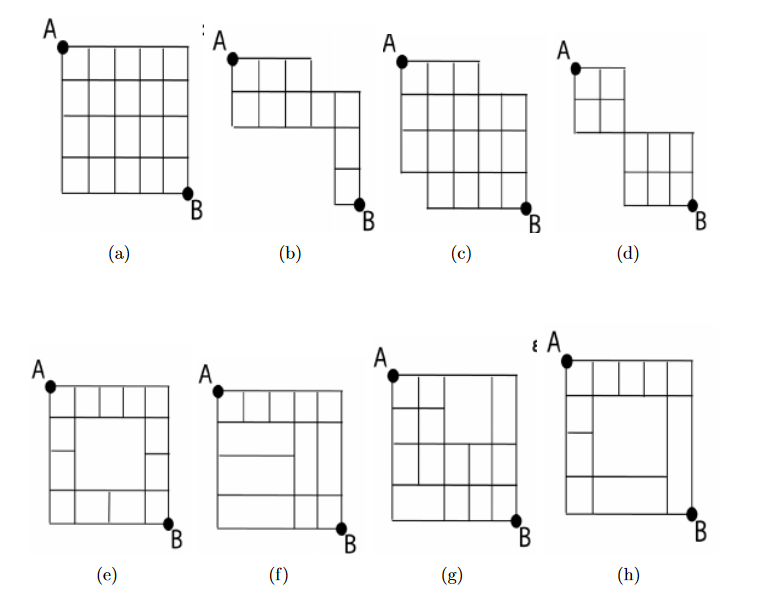
\includegraphics[scale=0.9]{Imagenes/IMG4/cuadricula_2.png}
    \end{center}






    
\end{problema}

    \begin{problema}
        Usando caminos, explica porqué es cierta la siguiente igualdad

        $$\binom{n}{k}=\binom{n}{n-k}$$
    \end{problema}


    \begin{problema}
        Usando caminos demuestra la identidad de pascal

        $$\binom{n+1}{k+1}=\binom{n}{k}+\binom{n}{k+1}$$ 
    \end{problema}


        \begin{problema}
        Demuestra usando caminos que 

        $$\binom{n}{2}=(n-1)+\binom{n-1}{2}.$$
    \end{problema}


    \begin{problema}
        Demuestra usando el modelo de caminos la siguiente identidad

        $$\binom{2n}{2}=2\binom{n}{2}+n^2.$$
    \end{problema}



    \begin{problema}
        Demuestra la identidad del presidente usando caminos $$(k+1)\binom{n+1}{k+1}=(n+1)\binom{n}{k}.$$

        Sugerencia: Puedes reescribir la identidad de la siguiente manera:$\binom{n+1}{k+1}\binom{k+1}{1}=\binom{n+1}{1}\binom{n}{k}.$
    \end{problema}


